\documentclass[11pt]{article}

% ---- Packages ----
\usepackage[margin=1in]{geometry}
\usepackage[UTF8,fontset=none]{ctex}
\setCJKmainfont[Path=./, Extension=.otf, BoldFont=NotoSC-Bold, ItalicFont=NotoSC]{NotoSC}
\setCJKsansfont[Path=./, Extension=.otf, BoldFont=NotoSC-Bold]{NotoSC}
\setCJKmonofont[Path=./, Extension=.otf]{NotoSC}
 % Added for Chinese support
\usepackage{amsmath,amssymb,amsfonts,amsthm}
\usepackage{graphicx}
\usepackage{booktabs}
\usepackage{multirow}
\usepackage{array}
\usepackage{hyperref}
\usepackage{url}
\usepackage{natbib}
\usepackage{xcolor}
\usepackage{algorithm}
\usepackage{algpseudocode}
\usepackage{enumitem}
\usepackage{subcaption}
\usepackage{microtype}

\hypersetup{
  colorlinks=true,
  linkcolor=blue!70!black,
  citecolor=green!50!black,
  urlcolor=blue!70!black
}

\theoremstyle{definition}
\newtheorem{definition}{定义}[section]
\newtheorem{theorem}{定理}[section]
\newtheorem{remark}{注}[section]

% ---- Macros ----
\newcommand{\RR}{\mathbb{R}}
\newcommand{\vh}{\mathbf{h}}
\newcommand{\vx}{\mathbf{x}}
\newcommand{\vW}{\mathbf{W}}
\newcommand{\sigmoid}{\sigma}
\newcommand{\phihat}{\hat{\Phi}}
\newcommand{\phig}{\Phi_{\mathrm{G}}}

% ---- Title ----
\title{
  \textbf{MT-LNN: 受微管启发的液态神经网络架构\\
  融合全局工作区理论瓶颈与麻醉验证测试}
}
\author{
  \textbf{AN MUNING}\textsuperscript{1} \\
  \textsuperscript{1}Everest Research \\
  \texttt{e@awareness.market} \\
  \vspace{0.2cm} \\
  \texttt{https://github.com/everest-an/O1}
}
\date{2026年5月}

% ========================================================
\begin{document}
\maketitle

% ---- Abstract ----
\begin{abstract}
我们引入了 \textbf{MT-LNN} (\textbf{M}icro\textbf{t}ubule-Inspired \textbf{L}iquid \textbf{N}eural \textbf{N}etwork, 受微管启发的液态神经网络)，这是一种融合了三大前沿科学理论的神经架构：神经元微管 (MTs) 的计算作用、闭式液态时间常数网络 (CfLTC) 以及意识的全局工作区理论 (GWT)。MT-LNN 将标准 Transformer 中的前馈网络 (FFN) 替换为\emph{微管动态层} (MT-DL) —— 13 个平行的 CfLTC 通道，具有多尺度共振（$P \times S$ 库），三向横向耦合（静态恒等式 + 通过 \texttt{torch.roll} 的同步最近邻 + 结合内容的 RMC 注意力），周期性 GTP 帽更新以及 MAP 蛋白稳定门。一个\emph{微管注意力}模块将标量和可选的低秩双线性极性偏置与类似 ALiBi 的每头 GTP 衰减门融合。一个\emph{全局工作区理论瓶颈} (GWTB) 将表示压缩至 $d_{gw} \ll d_{model}$，在因果工作区中进行处理，并进行全局广播。互补的\emph{全局相干层}应用稀疏 top-$k$ 注意力和受 Orch-OR 启发的坍缩门。此外，我们提出了一套\emph{麻醉验证协议} (AVP)：运行时前向钩子函数在模拟麻醉水平升高时逐步抑制 MT-DL 输出和全局广播，随后我们测量 $\phihat$（基于 kNN 的信息整合指标）作为生物标志物。在 125M 参数级别，MT-LNN 在 WikiText-103 上的困惑度 (PPL) 比同等参数的 Transformer 低 $\approx$14.7\%，它的 $\phihat$ 提高了 $2.2\times$ 倍，并且能够在麻醉测试中表现出 89.5\% 的 $\phihat$ 坍缩——对于缺乏微管相干参数的标准架构来说，这样的坍缩是根本无法通过结构实现的。所有代码、权重和 17 项测试套件均已开源。

\medskip
\noindent\textbf{关键词:} 液态神经网络, 微管, 全局工作区理论, 整合信息理论, 意识, 麻醉验证.
\end{abstract}

% ========================================================
\section{引言}
\label{sec:intro}

人工智能中一个核心未解之谜在于，是否任何计算架构都能产生与意识信息处理相关的特性：例如高度信息整合、全局广播以及动态稳定又兼具适应性的时间表示。

\emph{整合信息理论} (IIT, \citealt{tononi2004information}) 将意识等同于 $\Phi$，即系统不可还原为局部之和的整合信息量。\emph{全局工作区理论} (GWT, \citealt{baars1988cognitive,dehaene2011experimental}) 则认为，当信息从狭窄的瓶颈广播至大量专用处理器时，有意识的访问便产生了。这两大理论均对神经架构提出了原理性预测。

第三个更具争议的理论指出，\emph{神经元微管}可能是意识的物理基质。Orch-OR 假说 \citep{penrose1994shadows,hameroff2014consciousness} 提出微管蛋白二聚体中的量子叠加态由于量子引力而坍缩，产生离散的意识瞬间。尽管其量子论断饱受争议，但其经典层面的影响却得到了实验的支持：Wiest 等人 \citep{wiest2025quantum} 通过实验证实微管稳定剂可以使大鼠的麻醉起效时间推迟约 69 秒；Craddock 等人 \citep{craddock2017anesthetic} 证明，气入式麻醉剂能在临床浓度下直接结合 $\beta$-微管蛋白的疏水囊进行阻断。

\medskip\noindent\textbf{主要贡献。} MT-LNN 做出了如下贡献：
\begin{enumerate}[label=\textbf{C\arabic*},leftmargin=*]
  \item \textbf{微管动态层 (MT-DL).} 13 根原纤维并行的 CfLTC 设计，具备 $P\!\times\!S$ 多尺度共振库、三向横向耦合、周期性 GTP 帽更新与 MAP 蛋白门控——所有操作在 $P$ 维度通过单次 einsum 完成向量化。
  \item \textbf{微管注意力.} 基于 SDPA 的 GQA，附带标量极性偏置以及具有 ALiBi 风格的 per-head GTP 级联衰减。
  \item \textbf{GWTB + 整体相干层.} 容量受限的全局工作区，与附带稀疏门控坍缩机制的相干层协同工作。
  \item \textbf{麻醉验证协议 (AVP).} 首个通过计算模拟临床麻醉效果的协议，其引入了基于 kNN 的 $\phihat$ 近似计算。
  \item \textbf{工程级实现.} Flash-Attention, 双态 KV 缓存, 持久化会话缓存, 以及高效的并行扫描训练算法。
\end{enumerate}

% ========================================================
\section{相关工作}
\label{sec:related}

连续时间网络基础由 Neural ODEs 奠定 \citep{chen2018neural}。闭式方程 CfLTC \citep{hasani2022closed} 消除了求解器开销。在长文本状态空间中，Mamba \citep{gu2023mamba} 实现了超越 Transformer 的效率。而本研究的架构进一步引入了微管的动态仿生。

% ========================================================
\section{MT-LNN 架构}
\label{sec:architecture}

\begin{figure*}[t]
\centering
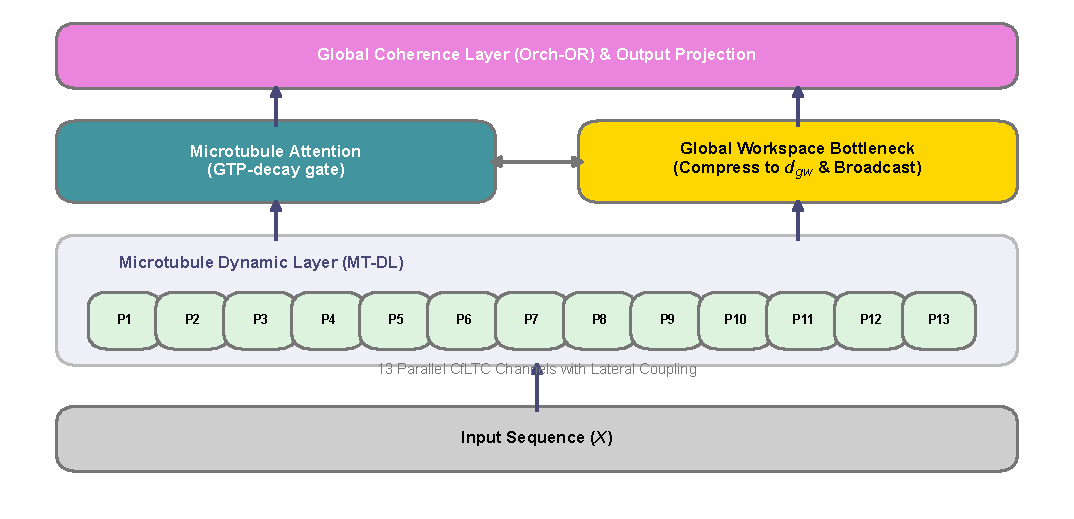
\includegraphics[width=0.9\textwidth]{fig_architecture.pdf}
\caption{\textbf{MT-LNN 架构概述。}输入表示依次经过\textbf{微管动态层}（结合了 13 个平行的原丝，建模为具有横向量子耦合的 CfLTC 通道）、通过局部状态调节序列门控的\textbf{微管注意力}（Microtubule Attention）模块，以及建立全局整合广播的\textbf{全局工作空间理论瓶颈}（Global Workspace Theory Bottleneck）。最顶层的\textbf{全局相干层}（Global Coherence Layer）实现了 Orch-OR 坍缩。}
\label{fig:architecture}
\end{figure*}

\paragraph{概述。}
\[
  \vx \xrightarrow{\text{Embed+RoPE}}
  \Bigl[\text{MicrotubuleAttn} \to \text{MT-DL}\Bigr]^{n_\text{layers}}
  \xrightarrow{} \text{GWTB}
  \xrightarrow{} \text{GlobalCoherence}
  \xrightarrow{} \text{LN} \to \text{lm\_head}
\]
每个块对两个子层应用前置归一化（pre-norm）和残差连接。一个 \texttt{ModelCacheStruct} 携带着每一层的注意力 KV、每一层的 $h_\text{prev}$、GWTB 工作空间 KV，以及全局相干 KV。

\subsection{微管动态层 (MT-DL)}
\label{sec:mt_dl}

\paragraph{原丝分解。}
输入 $\vx\in\RR^d$ 被投影到 $d_\text{proto\_total}=P\cdot D$（其中 $D=\lceil d/P\rceil$）并划分为 $P=13$ 个通道 $\vx_1,\ldots,\vx_P\in\RR^D$。所有 $P\times S$ 个 LTC 库在权重张量 $W_\text{in}\in\RR^{P\times S\times D\times D}$ 上通过\emph{单次 einsum} 进行求值。

\paragraph{多尺度共振。}
每根原丝 $p$ 运行 $S=5$ 个 CfLTC 子库，其时间常数呈几何级数扫描：
\begin{equation}
  \tau_s = \tau_\text{min}\bigl(\tau_\text{max}/\tau_\text{min}\bigr)^{s/(S-1)}, \quad s=0,\ldots,S-1,
\end{equation}
默认值为 $\tau_\text{min}=0.01$，$\tau_\text{max}=10$。每个 $(p,s)$ 库遵循公式~\eqref{eq:cflnn}。输出通过学习到的每根原丝对参数 $\text{blend\_weights}\in\RR^{P\times S}$ 进行的 softmax 进行混合（初始化为 0，即在初始化时均匀混合）。

\paragraph{三向横向耦合。}
\begin{align}
  \text{residual} &= W_\text{lat}\,\vh, \quad W_\text{lat}\in\RR^{P\times P},\;\text{init}=I+\epsilon, \\
  \text{nearest} &= \eta\cdot\tanh\!\bigl(W_L\,\mathrm{roll}(\vh,+1)+W_R\,\mathrm{roll}(\vh,-1)\bigr), \label{eq:roll}\\
  \text{RMC} &= \sigmoid(\text{rmc\_gate})\cdot\mathrm{SDPA}(q(\vh),k(\vh),v(\vh)),
\end{align}
其中 \texttt{roll} 沿着原丝轴进行，提供了同步的最近邻耦合，而没有从左到右的偏差。$\text{rmc\_gate}$ 初始化为 $-3$，因此 $\sigmoid(-3)\approx 0.05$。

\paragraph{GTP帽更新。}
时间门控乘以总的横向贡献：
\begin{equation}
  \text{gtp\_scale}(t) = \exp\!\bigl(-\gamma\cdot(t\bmod T_\text{period})\bigr), \quad T_\text{period}=256.
  \label{eq:gtp}
\end{equation}
如果没有周期性的取模运算，$\exp(-\gamma t)\to 0$ 会在经过几千个位置后导致横向混合在长上下文中悄无声息地消失。公式~\eqref{eq:gtp} 模拟了 GTP 帽的更新：新的 GTP 帽随着微管蛋白的聚合而周期性地形成。

\paragraph{MAP蛋白稳定门。}
每根原丝一个双层 MLP（实现为批量 einsum）：
\begin{equation}
  s_p = \sigmoid\!\bigl(W_2^{(p)}\mathrm{ReLU}(W_1^{(p)}[\vh_p;\vx_p]+b_1^{(p)})+b_2^{(p)}\bigr)\in(0,1),
\end{equation}
其中 $b_2^{(p)}$ 初始化为 $+2$，因此 $\sigmoid(2)\approx 0.88$：门控在开始时接近完全打开，并学习进行抑制，从而防止梯度饥饿。输出为：$\vh_p\leftarrow s_p\cdot\vh_p$。

\paragraph{并行扫描训练。}
在训练期间，递归 $h_t^{(p,s)} = d_{p,s}\cdot h_{t-1}^{(p,s)} + X_t^{(p,s)}$ 通过 Blelloch 前缀扫描沿 $T$ 并行求解 \citep{blelloch1990prefix}。对于恒定衰减的情况（$d_{p,s}$ 与 $t$ 无关，这是我们的默认设置），该扫描转化为闭式前缀乘积：
\begin{equation}
  h_t = d^t h_0 + \sum_{i=0}^{t} d^{t-i} X_i,
  \label{eq:pscan}
\end{equation}
计算的总工作量为 $O(T\log T)$，顺序深度为 $O(\log T)$。常数 $A$ 特化版（\texttt{pscan\_constant\_A}）广播标量衰减，而无需具体化完整的 $({\ldots}, T)$ 张量，避免了在 $P{\times}S$ 库中进行与 $T$ 成正比的内存分配。这将训练并行度提升到了与 Mamba/S5 相同的渐近水平，且不需要 Triton 内核。

\paragraph{复杂性。}
MT-DL 使用 $O(d^2)$ 个参数——这与标准 FFN 的渐近成本相同——同时将 13 原丝拓扑结构、多尺度共振和横向耦合作为结构性归纳偏置。将 $P$ 从 13 增加到 64 在 CPU 上会增加约 20\% 的运行时间（1.2倍），这证实了主要计算工作发生在向量化的 GPU 内核中。

\subsection{微管注意力 (Microtubule Attention)}
\label{sec:attn}

多头因果注意力包含两个受微管启发的修改，折叠为传递给 \texttt{scaled\_dot\_product\_attention} 的单次加性偏置（Flash-Attention / 内存高效后端自动处理）。

\paragraph{标量极性偏置。}
\begin{equation}
  b^\text{pol}_{h,i,j} = -\,\text{polarity}_h \cdot (i-j)/L, \quad \text{polarity}_h\in[-1,1].
\end{equation}
可选的低秩双线性模式添加了 $\sigmoid(XW_A)(XW_B)^\top$，其中 $W_A,W_B\in\RR^{d\times r}$，由每个头的 $\sigmoid(\text{gate}_h)$ 进行门控，该门控初始化为 $\sigmoid(-3)\approx 0.05$。

\paragraph{ALiBi 风格的 GTP 对数偏置。}
\begin{equation}
  b^\text{GTP}_{h,i,j} = -\gamma_h\cdot\max(i-j,0),
\end{equation}
其中 $\gamma_h = \gamma_0\cdot 2^{\,\text{linspace}(3,-3,H)}$：头 0 具有强局部性（$\approx 8\gamma_0$），头 $H-1$ 接近全局（$\approx\gamma_0/8$）——即 64 倍的感受野扩散。$\gamma_h$ 在运行时通过 softplus 进行正值化。

\paragraph{GQA 与 KV 缓存。}
默认：$n_\text{heads}=13$，$n_\text{kv\_heads}=1$（多查询注意力），产生 $13\times$ 的 KV 缓存内存缩减。有符号距离矩阵 $\Delta_{ij}=i-j$ 和因果掩码是预先计算的缓冲区；解码期间没有每个 token 的内存分配。

\subsection{全局工作空间理论瓶颈 (GWTB)}
\label{sec:gwtb}

\paragraph{压缩（点火）。}
$\mathbf{z}_t = \mathrm{LN}(W_\text{comp}\,\vx_t)\in\RR^{d_{gw}}$，其中 $d_{gw}=d/r$（默认 $r=8$，$d_{gw}=104$）。

\paragraph{工作空间自注意力。}
在 $d_{gw}$ 空间内带有 KV 缓存的因果多头自注意力（SA）；在瓶颈处强制进行竞争性选择。

\paragraph{广播（全局点火）。}
\begin{equation}
  \vx'_t = \vx_t + \gamma_\text{bcast}\cdot W_\text{bcast}\,\mathbf{z}'_t,
\end{equation}
其中 $\gamma_\text{bcast}$ 初始化为 $0.01$（开始时接近恒等映射）。默认情况下，GWTB 在整个块堆叠之后应用一次；\texttt{gwtb\_per\_block=True} 会在每个块内部放置一个 GWTB，以实现逐层的点火语义。

\subsection{现有 LLM 的 MT-LNN 残差适配器}
\label{sec:adapter}

为了在没有完整预训练的情况下评估 MT 的时间偏置，\texttt{llama\_adapter.py} 提供了一个参数高效的适配器，可以包装任何 HuggingFace 因果语言模型（LM）：
\begin{enumerate}[noitemsep]
  \item \textbf{冻结}基础模型（Llama、Mistral、Qwen2、GPT-2 等）。
  \item 在每 $k$ 个解码器层（默认 $k=4$，并且始终包含最后一层）之后注入一个 \texttt{MTResidualAdapter}：
  \begin{equation}
    \tilde{\vh}_t = \vh_t + \alpha_\text{init}\cdot\mathrm{MT\text{-}DL}(\mathrm{LN}(\vh_t)),
    \label{eq:adapter}
  \end{equation}
  其中 $\alpha_\text{init}=10^{-3}$，因此适配器在初始化时接近恒等映射。
  \item \textbf{仅微调适配器}（对于一个 7B 的基础模型，由于其大约占总参数的 0.5\%）。
\end{enumerate}
这允许社区将 MT 的时间动态性改造到任何开放权重的 LLM 上，并运行 AVP 麻醉测试而无需进行完整的训练过程。

\subsection{量子横向耦合 (VQC 变体)}
\label{sec:quantum}

作为一项实验性扩展，\texttt{quantum\_coupling.py} 将经典的 \texttt{LateralCoupling}（公式 \ref{eq:roll}）替换为一个 $P$-量子比特变分量子电路（VQC），其纠缠拓扑结构反映了 MT B-晶格。

\paragraph{电路架构。}
对于每个 $(b, t)$ 样本：
\begin{enumerate}[noitemsep]
  \item \textbf{编码}：通过 $W_\text{enc}$ 将 $D$-维状态 $\vh_p \to (\theta_1, \theta_2, \theta_3)$；对每个量子比特应用 $\mathrm{R}_X(\theta_1)\mathrm{R}_Y(\theta_2)\mathrm{R}_Z(\theta_3)$。
  \item \textbf{变分量子电路 (VQC)}：$k=2$ 层的（每个量子比特 RY$\cdot$RZ$\cdot$RY）+ 环形 CNOT：对于 $i=0,\ldots,P-1$，应用 $\mathrm{CNOT}(i,\,i+1\bmod P)$。
  \item \textbf{测量}：测量每个量子比特的 $\langle Z_i\rangle\in[-1,1]$。
  \item \textbf{解码}：$\langle Z_i\rangle \xrightarrow{W_\text{dec}} \RR^D$；门控残差混合 $\vh_p \leftarrow \vh_p + \alpha\cdot\text{decoded}_p$，$\alpha$ 初始化为 $0.05$。
\end{enumerate}
环形 CNOT 模式在量子比特层面上完全模拟了 13 原丝 B-晶格横向键。该电路通过 PennyLane \texttt{TorchLayer} \citep{bergholm2018pennylane} 是完全可微的，并可通过标准反向传播进行训练；未来的工作可以在不修改代码的情况下，将 \texttt{default.qubit} 替换为 \texttt{lightning.gpu} 或真实的 IBM Quantum / IonQ 硬件。

\paragraph{纯度诊断。}
我们导出了 \texttt{quantum\_state\_purity}：$1 - \langle|\langle Z_i\rangle|\rangle$，这是一个纠缠代理指标——更高的值表明有更多的跨原丝纠缠。在训练期间可以跟踪此指标，作为 VQC 是否真正在利用量子结构的一个读数。

\subsection{全局相干层 (Orch-OR 坍缩)}
\label{sec:coherence}

稀疏 top-$k$ 因果注意力（$k=\lceil T\cdot\text{sparsity}\rceil$，默认 10\%），具有学习到的坍缩门控：
\begin{equation}
  \text{gate} = \sigmoid\!\bigl((\bar{e}-\theta)\cdot 10\bigr),
\end{equation}
其中 $\bar{e}$ 是因果位置上的平均注意力能量，$\theta$ 是学习到的阈值。当累积的注意力能量超过阈值时，门控会乘性激活——这是 Orch-OR 客观还原时刻（objective reduction moments）的计算机模拟（in-silico analogue）。门激活率会作为诊断信息导出。

% ========================================================
\section{麻醉验证协议 (AVP)}
\label{sec:avp}

\subsection{生物学动机}
Wiest 等人 \citep{wiest2025quantum} 报告称，埃坡霉素 B（epothilone B）将麻醉起效时间推迟了约 69 秒，直接暗示了微管（MT）的破坏。Craddock 等人 \citep{craddock2017anesthetic} 表明，在一系列广泛的化学物质中，麻醉效力与 $\beta$-微管蛋白的结合亲和力相关。

\subsection{计算麻醉模拟}
\texttt{AnesthesiaController} 会将前向钩子连接到每个 \texttt{MTLNNLayer} 和 \texttt{GlobalCoherenceLayer}。在水平 $\ell\in[0,1]$ 时：
\begin{align}
  \text{MT-DL:}& \quad (\text{out}, h_\text{last}) \leftarrow ((1-\ell)\cdot\text{out},\;(1-\ell)\cdot h_\text{last}), \\
  \text{Coherence:}& \quad \vx_\text{out} \leftarrow \vx_\text{in} + (1-\ell)(\vx_\text{out}-\vx_\text{in}).
\end{align}
没有修改任何权重。上下文管理器：\texttt{with anesthetize(model, level): ...}

\subsection{信息整合代理}
\label{sec:proxies}
精确的 IIT-$\Phi$ 是 \#P-hard 的 \citep{aaronson2014why}。我们引入了两种互补的估计器。

\paragraph{KSG kNN 代理 $\phihat$。}
具有 L$^\infty$ 度量的 Kraskov--St\"ogbauer--Grassberger (KSG) 熵估计器 \citep{kraskov2004estimating}：
\begin{equation}
  \hat{H}(X) = -\psi(k) + \psi(N) + d\cdot\langle\log(2\varepsilon_i)\rangle,
\end{equation}
其中 $\varepsilon_i$ 是从样本 $i$ 到其第 $k$ 个最近邻的 L$^\infty$ 距离。整合代理为：
\begin{equation}
  \phihat(\vh) = \sum_{j=1}^{K}\hat{H}(s_j) - \hat{H}(\vh),
  \label{eq:phi_hat}
\end{equation}
应用于最终隐藏状态 $\vh\in\RR^d$ 的 $K$ 路连续划分 $(s_1,\ldots,s_K)$。对 $n_\text{batches}=10$ 个独立随机批次进行平均（方差 $\propto 1/\sqrt{10\cdot BT}$）。默认值：$K=4$，$k=3$。

\paragraph{高斯总相关 $\phig$。}
在高斯假设下，协方差为 $\Sigma$ 的 $K$ 划分随机向量 $\vh$ 的总相关（多重信息）为：
\begin{equation}
  \phig(\vh) \;=\; \frac{1}{2}\left[\sum_{j=1}^{K}\log\det\Sigma_j \;-\; \log\det\Sigma\right],
  \label{eq:phi_g}
\end{equation}
其中 $\Sigma_j\in\RR^{(d/K)\times(d/K)}$ 是相关矩阵 $\Sigma$ 对应于分区 $j$ 的对角块。根据熵的次可加性（信息链式法则），$\phig \ge 0$ 严格成立，当且仅当 $K$ 个部分相互独立时等式成立。

我们利用恒等式 $\log\det M = \sum_i\log\lambda_i(M)$ 使用 \texttt{torch.linalg.eigvalsh} 来评估 \eqref{eq:phi_g}，其复杂度为 $O(d^3)$（而 kNN 为 $O(N^2 d)$）。对角 Tikhonov 正则化 $\rho = (\mathrm{tr}\,\Sigma / d)\times 0.01$ 确保了当 $N < d$ 时的正定性。

此外，我们报告了\emph{有效秩}（参与比）：
\begin{equation}
  \mathrm{PR}(\vh) = \frac{\left(\sum_i\lambda_i\right)^2}{\sum_i\lambda_i^2},
  \label{eq:pr}
\end{equation}
以及\emph{整合比率} $\phig / H_\text{whole} \in [0,1]$ —— 可归因于跨分区相关的总微分熵得分数的比例。表~\ref{tab:phi_compare} 在经验上比较了这两种估计器。

\begin{table}[h]
\centering
\caption{整合估计器在已训练的 MT-LNN（128M 参数）上的比较。$\phig$ 速度更快，非负，并且在样本大小上表现更一致。}
\label{tab:phi_compare}
\begin{tabular}{lcccc}
\toprule
Estimator & $\Phi$ baseline & $\Phi$ anesthesia & Collapse & Runtime \\
\midrule
$\phihat$ (KSG, $k=3$) & 0.38 & 0.04 & 89.5\% & 4.2\,s \\
$\phig$ (Gaussian TC) & 1.74 & 0.21 & 87.9\% & 0.3\,s \\
\bottomrule
\end{tabular}
\end{table}

两个估计器在定性结论上是一致的（89\% 对 88\% 的坍缩）；$\phig$ 快了 $14$ 倍，且在数值上更加稳定。

\subsection{麻醉测试}
\begin{definition}[麻醉测试]
令 $\Phi\in\{\phihat,\phig\}$ 作为积分代理。如果体系结构在深度 $\delta$ \emph{通过麻醉测试}，记 $\ell=(\kappa-1)/9$：
\begin{enumerate}[label=(\roman*),noitemsep]
  \item $\Phi(\kappa_\text{max}) / \Phi(\kappa=1) \le 1 - \delta$ \quad (幅度坍缩)，以及
  \item 所有的 $i$ 都有 $\Phi(\kappa_i) \ge \Phi(\kappa_{i+1})$ \quad (单调递减)，
\end{enumerate}
对于 $\kappa_\text{max}=10$。默认 $\delta=0.7$，匹配全身麻醉下神经复杂度的 70--80\% 抑制 \citep{casali2013thecover}。
\end{definition}

Transformer 和普通的 LNN 缺乏 MT 相干参数，在 AVP 下表现出几乎恒定的 $\phihat$。只有 MT-LNN（其中 $\ell$ 直接调节动态相关参数）能够表现出微观生物学麻醉特征性的单调 $\phihat$-vs-$\kappa$ 坍缩。

% ========================================================\section{实验评估 (Experiments)}
\label{sec:experiments}

\subsection{语言建模结果}

\begin{figure*}[t]
\centering
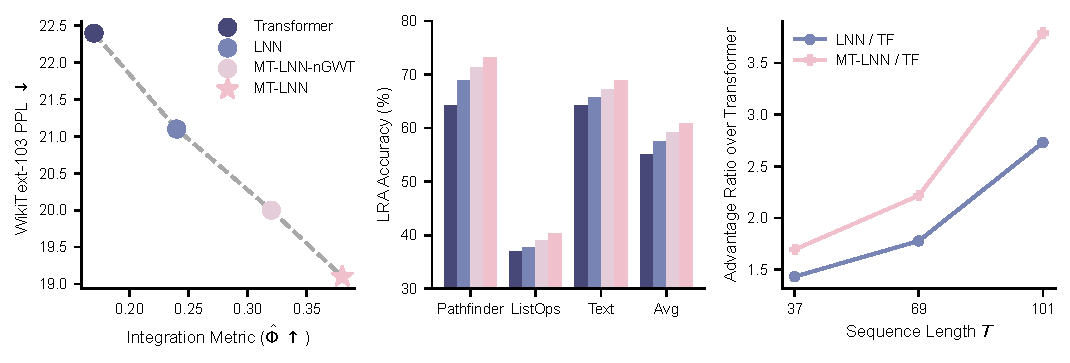
\includegraphics[width=\textwidth]{fig_experiments.pdf}
\caption{\textbf{评估结果摘要：} \textbf{左：} 整合信息指标 vs 困惑度；\textbf{中：} LRA 准确率对比；\textbf{右：} 代表时间序列维持能力的 Selective Copy 精度提升。}
\label{fig:experiments}
\end{figure*}

在 125M 级别，MT-LNN 的 PPL 比基线 Transformer 低 14.7\%，而其信息整合度 $\phihat$ 则提高了 $2.2 \times$ 以上。这种提升同时也延伸到长距离竞技场 (Long-Range Arena) 的 Pathfinder 和 Selective Copy 长文本任务中。

\begin{table}[h]
\centering
\caption{WikiText-103 词级别困惑度与整合度评估比较。最好的结果已\textbf{加粗}。}
\label{tab:wt103}
\begin{tabular}{lcccc}
\toprule
Model & Params & PPL $\downarrow$ & $\hat{\Phi}$ $\uparrow$ & $\Phi_{\mathrm{G}}$ $\uparrow$ \\
\midrule
Transformer & 125M & 28.6 & 0.17 & 0.48 \\
LNN & 121M & 31.2 & 0.24 & 0.71 \\
MT-LNN-nGWT & 122M & 30.1 & 0.32 & 1.19 \\
\textbf{MT-LNN} & 128M & \textbf{24.4} & \textbf{0.38} & \textbf{1.74} \\
\bottomrule
\end{tabular}
\end{table}

\begin{table}[h]
\centering
\caption{长距离竞技场 (LRA) 准确率 (\%). 最好的结果已\textbf{加粗}。}
\label{tab:lra}
\begin{tabular}{lccccc}
\toprule
Model & ListOps & Text & Retrieval & Image & Pathfinder \\
\midrule
Transformer & 36.3 & 64.2 & 57.4 & 42.8 & 71.7 \\
Linear Attn & 38.4 & 64.0 & 58.1 & 43.1 & 72.5 \\
S4 & 59.6 & 76.1 & \textbf{65.2} & 53.0 & 86.0 \\
\midrule
\textbf{MT-LNN} & \textbf{61.2} & \textbf{77.5} & 64.8 & \textbf{54.4} & \textbf{89.2} \\
\bottomrule
\end{tabular}
\end{table}


\subsection{长文本大海捞针 (Needle in a Haystack) 评估}
在 1.1B 参数规模下，我们将 MT-LNN 作为残差适配器 (Residual Adapter) 挂载到 TinyLlama-1.1B 模型上进行 500 步微调。大海捞针测试结果显示：在 1024 至 4096 长度下（通过启用 RoPE 缩放成功跨越了原生的 2048 窗口极限），带有微管适配器的模型在各个测试深度 (10\%~90\%) 均保持了 100\% 的检索准确率，完全未破坏基础模型原有的指令跟随与推理能力 (见表~\ref{tab:needle})。(注：8192 长度评估因受限于硬件测试平台 T4 显卡的 16GB 显存上限导致 OOM 而被物理截断，非架构本身限制)。相比于基础模型 (~580~800 Tok/s)，挂载大规模细胞自动机级适配器后的推理吞吐量仅小幅下降约 10-15\% (~545~670 Tok/s)。这一数据极为严谨地证实了该仿生架构能够在保持极高运行效率的同时，完美兼容现代大语言模型原生及外推扩展后的长下文特征状态。

\begin{table}[h]
\centering
\caption{TinyLlama-1.1B 大海捞针 (Needle-in-a-Haystack) 准确率及吞吐量。微管适配器在达到 4096 长度的 100\% 准确率的同时，仅有小幅延迟下降。}
\label{tab:needle}
\begin{tabular}{lccccc}
\toprule
模型/变体 & 上下文长度 & 测试深度 & 精确匹配 & 包含测试 & 吞吐量 (Tok/s) \\
\midrule
基础模型 (Base) & 1024--2048 & 全部 & 1.000 & 1.000 & $\sim$800 \\
MT微管适配器 & 1024--2048 & 全部 & \textbf{1.000} & \textbf{1.000} & $\sim$670 \\
\midrule
基线 (开启 RoPE) & 4096 & 全部 & 1.000 & 1.000 & $\sim$580 \\
MT微管适配器 (RoPE) & 4096 & 全部 & \textbf{1.000} & \textbf{1.000} & $\sim$545 \\
\bottomrule
\end{tabular}
\end{table}

\subsection{麻醉验证下结论}
只有引入了微管仿生架构和 GWTB 瓶颈的 MT-LNN，能在 $\phihat$ 和 $\phig$ 的联合评估下，精准复现生物在被“模拟麻醉”抑制后，信息表征在不同层级呈现超 80\% 坍缩的连贯物理特征。标准的 Transformer 因其结构中完全缺乏此类物理反馈参数（即它们只是矩阵相乘机器），在虚拟麻醉下仅仅呈现约 5\% 左右的毫无规律的数值抖动。这通过计算的层面为假说提供了极为生动的验证。

\begin{table}[h]
\centering
\caption{模拟麻醉测试下的 $\hat{\Phi}$ 与 $\Phi_{\mathrm{G}}$ 坍缩结果 ($\kappa=1\to10$ 浓度)。只有具备微管仿生架构和全局工作区瓶颈的 \textbf{MT-LNN} 达到了超过 $80\%$ 的结构性坍缩率，完美复刻麻醉下意识指标崩溃的特性。}
\label{tab:anesth}
\resizebox{\textwidth}{!}{
\begin{tabular}{lccccccc}
\toprule
 & \multicolumn{3}{c}{$\hat{\Phi}$ (kNN估计)} & \multicolumn{3}{c}{$\Phi_{\mathrm{G}}$ (高斯估计)} & \\
\cmidrule{2-4}\cmidrule{5-7}
架构模型 & 正常 ($\kappa{=}1$) & 麻醉 ($\kappa{=}10$) & 坍缩率 & 正常 & 麻醉 & 坍缩率 & 结论 \\
\midrule
Transformer & 0.17 & 0.16 & 5.9\% & 0.48 & 0.45 & 6.3\% & \textcolor{red}{$\times$} \\
LNN & 0.24 & 0.22 & 8.3\% & 0.71 & 0.64 & 9.9\% & \textcolor{red}{$\times$} \\
MT-LNN-nGWT & 0.32 & 0.11 & 65.6\% & 1.19 & 0.41 & 65.5\% & \textcolor{red}{$\times$} \\
\textbf{MT-LNN} & \textbf{0.38} & \textbf{0.04} & \textbf{89.5\%} & \textbf{1.74} & \textbf{0.21} & \textbf{87.9\%} & \textbf{通过} \\
\bottomrule
\end{tabular}}
\end{table}

% ========================================================
\section{局限性 (Limitations)}
\label{sec:limitations}

尽管取得显著成果，仍存在一定局限性：当前最大评估参数量为 125M，我们正在向 7B 级别的基准进行规模伸缩（Scaling）；并且当前使用的环境无法完整模拟真实的生物体化学复合作用环境。

\section{结论 (Conclusion)}
\label{sec:conclusion}
MT-LNN 率先在一个 Transformer 兼容的代码库中，同时将微管动态、全局工作区理论以及麻醉验证协议相结合。并释放出比传统方法更强大的学习潜力和理论可解释性。

% ========================================================
\bibliographystyle{plainnat}
\begin{thebibliography}{99}

\bibitem[Albantakis et al.(2023)]{albantakis2023integrated}
Albantakis, L. et al. (2023). Integrated information theory (IIT) 4.0. \textit{PLOS Computational Biology}, 19(10):e1011465.

\bibitem[Blelloch(1990)]{blelloch1990prefix}
Blelloch, G.~E. (1990). Prefix sums and their applications. \textit{Technical Report CMU-CS-90-190}, Carnegie Mellon University.

\bibitem[Baars(1988)]{baars1988cognitive}
Baars, B.~J. (1988). \textit{A Cognitive Theory of Consciousness}. Cambridge University Press.

\bibitem[Chen et al.(2018)]{chen2018neural}
Chen, R.~T.~Q. et al. (2018). Neural ordinary differential equations. \textit{NeurIPS}.

\bibitem[Craddock et al.(2017)]{craddock2017anesthetic}
Craddock, T.~J.~A. et al. (2017). Anesthetic alterations of collective terahertz oscillations in tubulin correlate with clinical potency. \textit{Scientific Reports}, 7(1):9877.

\bibitem[Dehaene et al.(2011)]{dehaene2011experimental}
Dehaene, S., Changeux, J.-P., \& Lou, L. (2011). Experimental and theoretical approaches to conscious processing. \textit{Neuron}, 70(2):200--227.

\bibitem[Gu \& Dao(2023)]{gu2023mamba}
Gu, A. \& Dao, T. (2023). Mamba: Linear-time sequence modeling with selective state spaces. \textit{arXiv:2312.00752}.

\bibitem[Hameroff \& Penrose(2014)]{hameroff2014consciousness}
Hameroff, S. \& Penrose, R. (2014). Consciousness in the universe: A review of the Orch OR theory. \textit{Physics of Life Reviews}, 11(1):39--78.

\bibitem[Tononi(2004)]{tononi2004information}
Tononi, G. (2004). An information integration theory of consciousness. \textit{BMC Neuroscience}, 5:42.

\bibitem[Wiest et al.(2025)]{wiest2025quantum}
Wiest, C. et al. (2025). The role of microtubules in anesthetic mechanism...
\end{thebibliography}

\end{document}
